\documentclass[a4paper,openright,12pt]{article}
%\documentclass[journal]{IEEEtran}
\usepackage[activeacute,spanish]{babel} 
\usepackage{multirow}
\usepackage[utf8]{inputenc}
\usepackage{graphicx}
\usepackage{lscape}
\usepackage{lmodern}
\usepackage{listings}
\usepackage{color}
\usepackage{hyperref}
%\usepackage[left=2.5 cm,right=2cm,top=2.5 cm,bottom=2cm]{geometry}
\usepackage{graphicx} 
\usepackage{pdfpages}
\usepackage{anysize}
% Salto de línea tras título de secciones \paragraph
\makeatletter % necesario para que reconozca a '@' como carácter normal
\renewcommand{\paragraph}{\@startsection{paragraph}{4}{\z@}{-3.25ex \@plus
-1ex \@minus -.2ex}{1.5ex \@plus .2ex}{\normalfont\normalsize\bfseries}}
\makeatother % necesario para que restablezca '@' como carácter especial

% Salto de línea tras título de secciones \paragraph
\makeatletter % necesario para que reconozca a '@' como carácter normal
\renewcommand{\subparagraph}{\@startsection{subparagraph}{4}{\z@}{-3.25ex \@plus
-1ex \@minus -.2ex}{1.5ex \@plus .2ex}{\normalfont\normalsize\bfseries}}
\makeatother % necesario para que restablezca '@' como carácter especial


\begin{document}
\renewcommand{\tablename}{Tabla}
\renewcommand{\listtablename}{Índice de tablas}
\renewcommand{\thesection}{\Alph{section}}
\renewcommand{\thesubsection}{\arabic                                                                                                                                                                                                                                                                                                                               {subsection} }

%lista de figuras 
\renewcommand\listfigurename{Índice de figuras}

\setcounter{secnumdepth}{5}
\setcounter{tocdepth}{5}
%\renewcommand{\labelenumi}{\Alph{enumi}.}
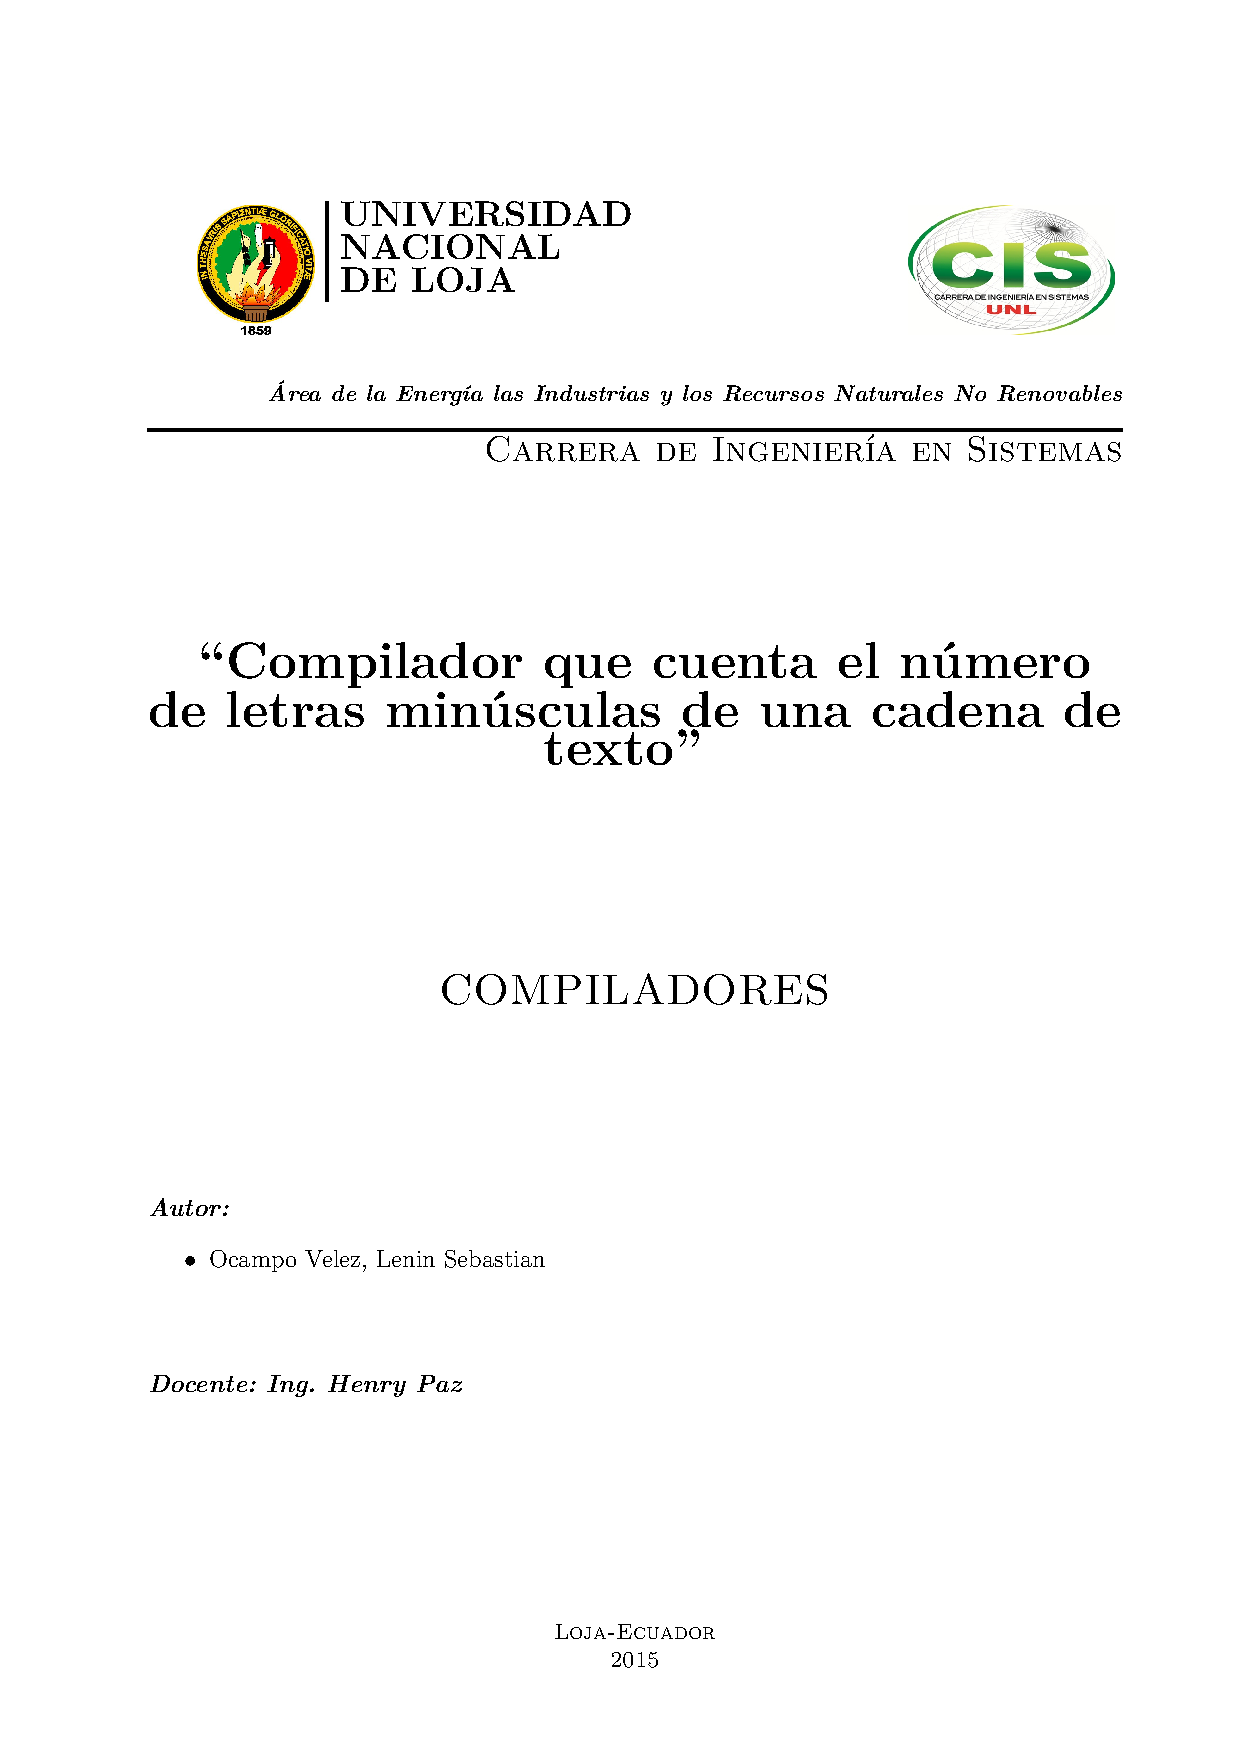
\includepdf[pages={1}]{portadaCis.pdf}

\marginsize{3cm}{2cm}{2cm}{2cm}

\newpage
\tableofcontents
\newpage
%\listoftables
%\listoffigures
\newpage
\vspace*{7 cm}
\begin{center}
\section{Tema}
\begin{Huge}
\textbf {“Compilador que cuenta el número de letras minúsculas de una cadena de texto”}
\end{Huge}
\end{center}



\newpage
\section{Introducción}

Para la realización del trabajo me base en la creación de un lenguaje a partir de un alfabeto con el objetivo de crear palabras claves, identificadores, caracteres(letras a-z).
Para validar lo anteriormente mencionado  utilizamos las herramientas:
Jflex: cuyo propósito es el de facilitar la construcción del analizador léxico. Para el analizador sintáctico utilizamos la herramienta CUP donde se realizo la integración con Jflex para la creación del compilador, también se utilizo la herramienta Jflap para la experimentación de lenguajes formales, la validación de las expresiones regulares, leer el flujo de caracteres de entrada  y transfórmalos en una secuencia de componentes léxicos.\\
Dicho problema fue planteado en base a la necesidad de crear un compilador especifico, que se encargue de verificar la parte léxica y sintáctica  de la cadena de texto. Comprendiendo así el funcionamiento y estructura de cada uno de los analizadores tanto léxico como sintáctico.

\section{Descripción}

Dentro del tema planteado “Analizador Léxico, sintáctico que cuenta el numero de letras minúsculas de una cadena de texto”, se pide al usuario que ingresa un texto cuyo formato esta establecido, esta cadena debe ser escrita dentro de dos paréntesis, Ejm: (xyz@gmail.com) y para que la cadena sea valida se debe especificar el símbolo “;” como fin de linea, que indica que hasta esa columna se ingreso el texto o cadena a la cual se desea contar el numero de letras.\\
También dentro del ejemplo se especifica que los números Ejm: (098765) y caracteres especiales  Ejm: (@\#)  no serán tomados en cuenta, ya que solo se pretende calcular el numero de letras minúsculas.

\subsection{EJEMPLO}

\textbf{ENTRADA DEL TEXTO O CADENA:}
\\

(ocampolenin);(leninsebastian1992);
\\
\textbf{SALIDA POR CONSOLA:}\\

CADENA en Linea 1 Columna 2 CADENA: ocampolenin\\
Letras Encontradas: 11\\
Error Lexico: Linea 1 Columna 30<1> \\
Error Lexico: Linea 1 Columna 31<9> \\
Error Lexico: Linea 1 Columna 32<9> \\
Error Lexico: Linea 1 Columna 33<2> \\
CADENA en Linea 1 Columna 16 CADENA: leninsebastian\\
Letras Encontradas: 14\\


Palabras Reservadas\\

“(”  especifica el símbolo reservado con la que inicia la sentencia y posterior el texto o cadena.\\
“)”  especifica el símbolo reservado de cierre, delimita hasta donde se debe ingresar el texto o cadena.\\
“;”  especifica el fin de la sentencia y permite el ingreso de otra cadena con el mismo formato.


\section{Automata del Compilador}

Para la creación de nuestro AFD, utilizamos la herramienta JFlap (ver Figura 1), la misma que nos facilitó la validación de las expresiones regulares establecidas en el analizador sintactico.
\begin{center}
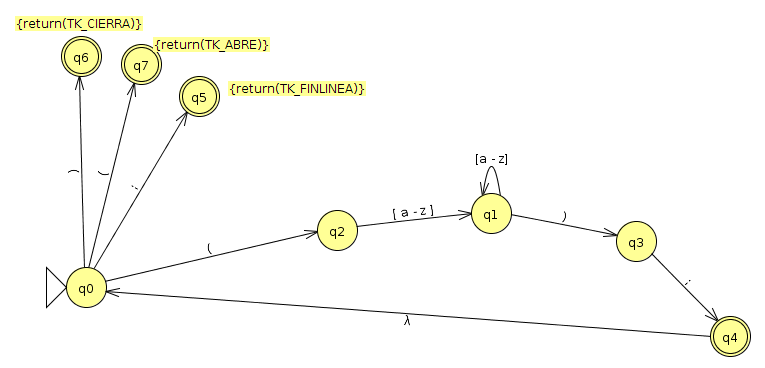
\includegraphics[height=0.37\textheight]{automata.png}
Figura 1: Autónoma Finito Determinista
\end{center}
\section{Analizador Léxico Archivo lexer.flex}

Habitualmente el termino "análisis léxico" se refiere al tratamiento de la entrada que produce como salida la lista de tokens. Un token hace alusión a las unidades mas simples que tiene significado. Habitualmente un token o lexema queda descrito por una expresión regular. El termino Léxico viene del griego lexis, que significa "palabra". Sin embargo, en el análisis léxico, ultima posición en la que se produjo un emparejamiento y que es aceptada por una de las expresiones regulares que definen los lexemas del lenguaje dado.\cite{1}\\

A continuación se explicara de una manera mas detallada la estructura del archivo .flex y como esta
definida su estructura para el compilador planteado.

\subsection{Codigo de Usuario}

\begin{center}
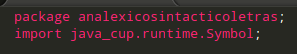
\includegraphics[height=0.05\textheight]{usuario.png}
\\
Figura 2: Importaciones
\end{center}

En esta sección se incluyen las construcciones para indicar que las clases Java generadas a partir de este fichero pertenecen a un determinado package o importar las clases Java necesarias. Para ambas cosas se utiliza exactamente la misma sintaxis que en Java. Esta parte contendrá como mínimo la siguiente línea:\\

import java\_cup.runtime.Symbol; \\
Nótese que puesto que las clases java generadas por CUP importan las clases del paquete java\_cup.runtime, el directorio donde se encuentre este paquete deberá estar en el classpath tanto al compilar las clases como al ejecutar un programa en Java que las use (este paquete está incluido en las clases de CUP).\\


\subsection{Directivas}

\begin{center}
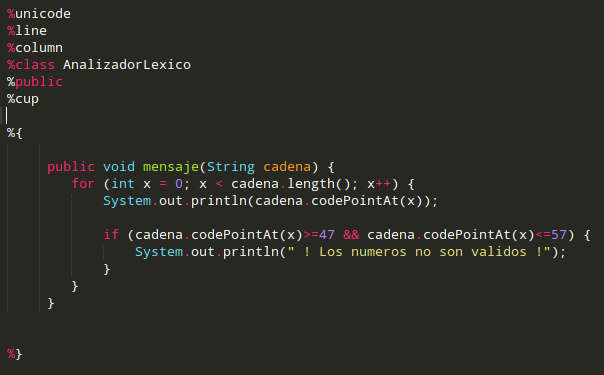
\includegraphics[height=0.4\textheight]{directivas.png}
\\
Figura 3: Directivas
\end{center}

La linea 1: de codigo \textbf{\%unicode} brinda un soporte completo con caracteres unicode.\\
La linea 2: \textbf{\%line:} agrega la variable int yyline, para indicar la fila del lexema.\\
La linea 3: \textbf{ \%column}  agrega la variable int yycolumn, para indicar la columna del lexema.\\
La linea 4: \textbf{ \%class}  especifica en nombre de la clase en este caso AnalizadorLexico.\\
La linea 5: \textbf{ \%public}  especifica una clase publica.\\
La linea 6: \textbf{ \%cup}  especifica la compatibilidad con cup.\\

A continuación se es especifica el código entre \%\{ y \%\}, el cual representa el código java que sera copiado en el analizador léxico.\\

En este caso existe un método que emite un error o advertencia al 
momento de ingresar un numero, este método utiliza el código ASCII, para
determinar que se encuentra entre el rango de los números reales, este método
emite un mensaje en caso de comprobarse que es un numero: ! Los números no son validos !


\subsection{Reglas para Expresiones Regulares}

\begin{center}
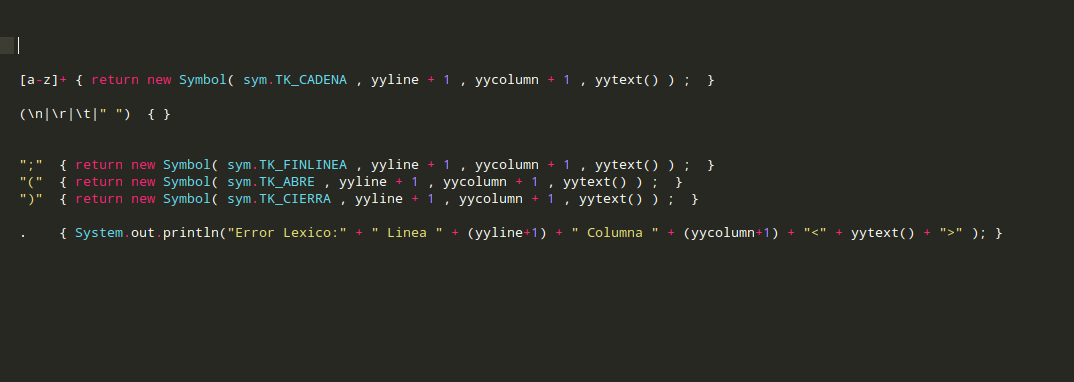
\includegraphics[height=0.25\textheight]{expres.png}
\\
Figura 4: Reglas
\end{center}

Esta seccion contiene expresiones regulares y acciones. Las acciones son código en Java que se ejecutara cuando se encuentre una entrada valida para la expresion regular correspondiente.\\

YYINITIAL es el estado inicial del analizador lexico al escanear.\\

En la linea 1: La cerradura positiva [a-z]+ nos dice que siempre va a existir una letra o muchas letras, es decir se pretende insertar una cadena de texto no importa el tamaño. Establece el token Tk\_Cadena , luego establece los métodos yyline y yycolumn  como ya sabemos para establecer la line y columna del token.\\

En la linea 2:  Se especifica que no se toma en cuenta los espacios, espacio en blanco, salto de carro, tabulador, salto de linea.\\


La linea 3: ";" especifica el token fin de linea es decir el símbolo que determina el final de la expresión.\\
La linea 4: "(" especifica el token el paréntesis de apertura.\\
La linea 5: ")" especifica el token el paréntesis de cierre.\\
La linea 6: . Especifica que los caracteres especiales se tomaran como un error lexico.\\




\section{Analizador Sintáctico Archivo parser.cup}

A continuacion se explica una breve descripción de algunos de los elementos soportados por CUP. Existen muchas opciones o funcionalidades de CUP .

\subsection{Definición de paquete y sentencias import.}

\begin{center}
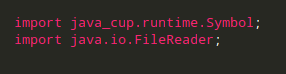
\includegraphics[height=0.08\textheight]{parser1.png}
\\
Figura 5: Importaciones cup
\end{center}

Esta parte contendrá como mínimo la siguiente línea:\\

import java\_cup.runtime.*;\\ \\

Importaciones del parser.cup \\

import java\_cup.runtime.Symbol;\\
import java.io.FileReader; Importacion de la clase FileReader que permite leer archivos.\\ \\
Nótese que puesto que las clases java generadas por CUP importan las clases del paquete java\_cup.runtime, el directorio donde se encuentre este paquete deberá estar en el classpath tanto al compilar las clases como al ejecutar un programa en Java que las use (este paquete está incluido en las clases de CUP).


\subsection{Sección de código de usuario}

\begin{center}
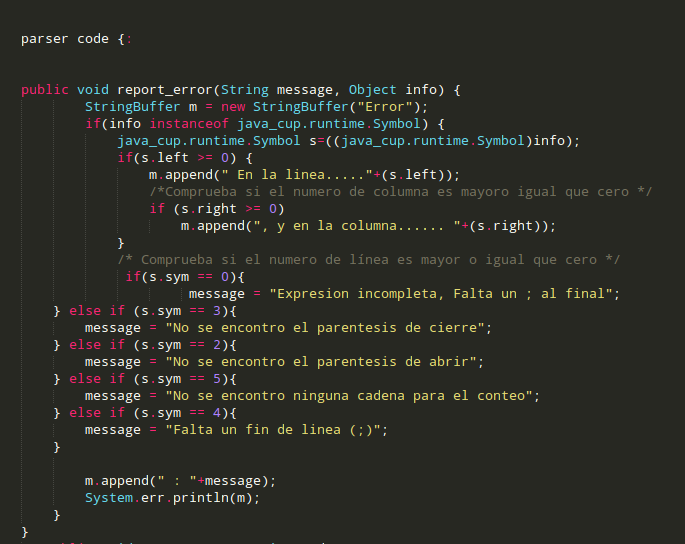
\includegraphics[height=0.5\textheight]{parser.png}
\\
Figura 6: parser code cup
\end{center}

En esta sección se puede incluir código Java que el usuario desee incluir en el analizador sintáctico que se va a obtener con CUP. Existen varias partes del analizador sintáctico generado con CUP en donde se puede incluir código de usuario. Aquí vamos a ver solamente una de ellas. La declaración:\\

parser code \{:\\
...\\
:\};\\
permite incluir código Java en la clase parser, generada por CUP. Como veremos más adelante, se pueden redefinir aquí los métodos que se invocan como consecuencia de errores de sintaxis.\\


En la Figura 5: Importaciones cup se observa el método report\_error este permite
determinar específicamente la linea y columna donde se encuentra el error sintáctico, para determinar con exactitud el tipo de error según la expresión
utilizamos el método sym para obtener un entero que es el identificador de la 
palabras o símbolos reservados, se realiza un if-else anidado haciendo la comparación y especificando el mensaje según el error.
Por ultimo se imprime por consola el error, con el método System.err.\\


\textbf{sym: } identifica cuál es el símbolo terminal o no terminal representado por el objeto. A cada símbolo terminal y no terminal definidos en el documento se les asocia un número diferente que le identifica.\\

\textbf{value: } si el objeto de la clase Symbol representa un símbolo terminal o no terminal que tenga asociado un objeto Java, dicho objeto se guarda en el atributo value.\\

\textbf{left y right: } aunque su uso no es imprescindible, habitualmente se utilizan para identificar la línea de texto en la que comienza (left) y termina (right) la parte del programa que se corresponde con ese símbolo terminal o no terminal. Se usan cuando se produce un error de sintaxis para indicar el lugar donde se encuentra el error.

\begin{center}
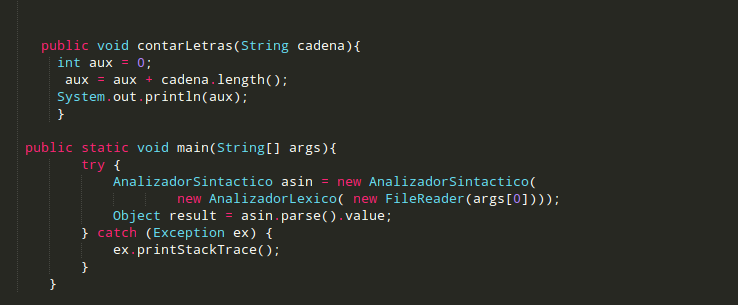
\includegraphics[height=0.3\textheight]{parser2.png}
\\
Figura 7: parser code cup
\end{center}

El método contarLetras es especifico de mi compilador, este método
me permite recibir una cadena de texto, como se explico anteriormente
la cadena que recibirá el método solo se encontraran letras minúsculas
ya que mi analizador léxico solo permite el alfabeto [a-z];\\

Luego se crea el método estático main para inicializar el Analizador
Léxico y por consiguiente inicializar el Analizador Sintáctico.


\subsection{Declaración de símbolos terminales y no terminales}

En esta sección se declaran los símbolos terminales y no terminales de la gramática que define el analizador sintáctico que deseamos producir. Tanto los símbolos no terminales como los símbolos terminales pueden, opcionalmente, tener asociado un objeto Java de una cierta clase. Por ejemplo, en el caso de un símbolo no terminal, esta clase Java puede representar los subárboles de sintaxis abstracta asociados a ese símbolo no terminal. En el caso de los símbolos terminales (o Tokens), el objeto Java representa el dato asociado al Token (por ejemplo un objeto de la clase Integer que represente el valor de una constante, o un String que represente el nombre de un identificador).\cite{2}


\begin{center}
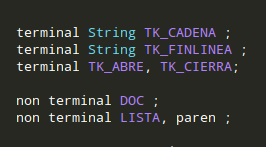
\includegraphics[height=0.17\textheight]{terminales.png}
\\
Figura 8: Símbolos terminales y no terminales
\end{center}

Linea 1 y 2: podemos ver definiciones de terminales que tienen un objeto Java asociado como String TK\_CADENA y  TK\_FINLINEA que devuelven un texto plano.\\

Linea 3: podemos ver definiciones de terminales que no tienen ningún objeto Java asociado como TK\_ABRE, TK\_CIERRA, que especifican la apertura y cierre de los paréntesis y dentro debe estar la cadena.\\

Linea 5: y 6 Las definiciones de símbolos no terminales que no tienen un objeto Java asociado como DOC, LISTA, paren.


\subsection{Definición del símbolo inicial de la gramática y las reglas de producción}
\begin{center}
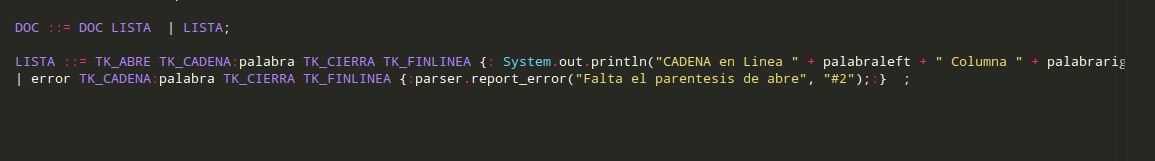
\includegraphics[height=0.13\textheight]{terminales2.png}
\\
Figura 9: Gramática cup
\end{center}

Linea1: Se establece la primera regla de producción, donde tenemos un símbolo no terminal como antecedente, en este caso  se establece DOC, seguido de ::= y las reglas de producción que le tengan como antecedente, en este caso DOC LISTA | LISTA, separadas por el símbolo | . Después de la última regla de producción se termina con punto y coma.\\

Linea2: Se establece la primera regla de producción, donde tenemos un símbolo no terminal como antecedente, en este caso es LISTA, seguido de ::= y a continuación las reglas de producción que le tengan como antecedente, en la figura 9 se observa un símbolo no terminal TK\_ABRE, que especifica que debe haber un paréntesis de apertura, seguido otro símbolo no terminal TK\_CADENA:palabra que es donde se guarda el texto de la cadena, seguido otro símbolo no terminal TK\_CIERRA , que especifica que debe haber un paréntesis de cierre, seguido otro símbolo no terminal TK\_FINLINEA , seguido entre {: ... :} se incluye el código Java donde se encuentra un método de salida por consola donde muestra el texto de la cadena, ubicación linea y columna, seguido se encuentra el método contarletras() declarado en el parser que devuelve el numero de letras minúsculas del texto. Para finalizar se especifica que debe haber un punto y coma al final de la expresión, separadas por el símbolo | . Después de la última regla de producción se termina con punto y coma.

\section{Resultados}
A continuación se muestran los resultados del compilador, ejecutamos la clase principal
Main.java y nos muestra la siguiente salida por consola.


\begin{center}
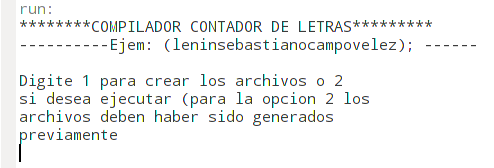
\includegraphics[height=0.2\textheight]{resultados.png}
\\
Figura 10: Salida Consola Main.java
\end{center}

La salida por consola de la clase Main.java da un ejemplo como se debe ingresar los datos, la siguiente sentencia nos pide digitar 1 para crear las clases AnalizadorLexico.java y AnalizadorSintactico.java, estos archivos son generados en base a los archivos lexer.flex
y parser.cup según el ejemplo.\\
La opción 2 es para ejecutar el compilador, pero se debe tener en cuenta que los archivos deben ya estar creados con la opción 1.

\subsection{Archivo de Entrada entrada.txt}

\begin{center}
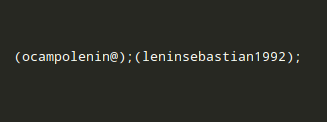
\includegraphics[height=0.15\textheight]{entrada.png}
\\
Figura 11: Archivo de entrada
\end{center}

En la figura 11: Archivo de entrada se observa un caso de prueba del compilador donde se especifica lo siguiente: existen dos cadenas ingresadas, ya que existen dos final de linea con el símbolo ; y dentro de paréntesis como lo especifica las expresiones regulares.\\
En este caso se  ingresan dos cadenas ya que como se especifico en el analizador léxico no se tomaran en cuenta los numeros y caracteres especiales : \\
  (ocampolenin@);(leninsebastian1992);\\
La primera:  ocampolenin\\
La segunda:  leninsebastian1992\\


\subsection{Salida por consola Compilador}

\begin{center}
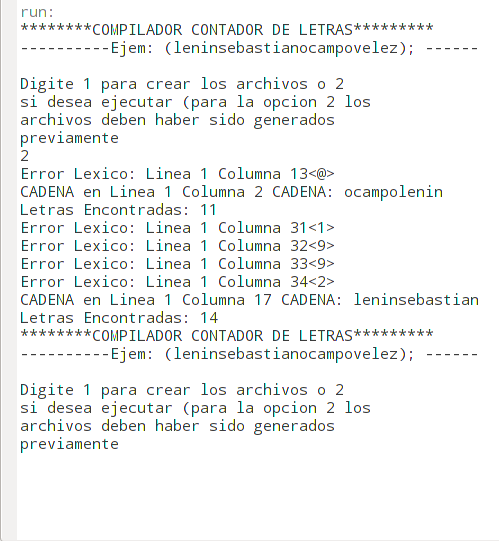
\includegraphics[height=0.5\textheight]{salida.png}
\\
Figura 12: Salida por Consola
\end{center}


En la figura 12: Salida por Consola se muestra la ejercicio del compilador, donde analiza la parte léxica, sintáctica y semántica.\\

Linea1 de la salida por consola: Muestra un error Léxico en la Linea 1 Columna 13 y especifica el valor del objeto, en este caso es @ ya que no se permiten caracteres especiales.\\

Linea2 de la salida por consola: Muestra que encontró una cadena en la linea 1 columna 2 y especifica el valor del objeto, en este caso: ocampolenin.\\

Linea3 de la salida por consola: Muestra el numero de letras encontradas en la cadena donde se ocupa el método contarLetras() de la clase AnalizadorSintactico.java que devuelve el numero de letras minúsculas encontradas en la cadena. \\

Linea4 de la salida por consola:  muestra error léxico por un numero.\\

Linea5 de la salida por consola:  muestra error léxico por un numero.\\

Linea6 de la salida por consola:  muestra error léxico por un numero.\\

Linea7 de la salida por consola:  muestra error léxico por un numero.\\

Linea8 de la salida por consola: Muestra que encontró una cadena en la linea 1 columna 17 y especifica el valor del objeto, en este caso: leninsebastian.\\

Linea9 de la salida por consola: Muestra el numero de letras encontradas en la cadena donde se ocupa el método contarLetras() de la clase AnalizadorSintactico.java que devuelve el numero de letras minúsculas encontradas en la cadena. 

\subsection{Errores}

\begin{center}
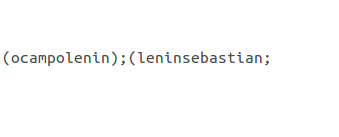
\includegraphics[height=0.15\textheight]{entradaerror.png}
\\
Figura 13: Entrada error sintáctico sin parentesis
\end{center}


En la figura 13: Se muestra la entrada o la cadena ingresada la cual tiene un error sintáctico como se especifico en las expresiones regulares cuyo formato es la cadena entre paréntesis y por ultimo un símbolo ; para especificar el final de la cadena. En este caso se observa que la segunda cadena no tiene  el paréntesis de cierre, por lo tanto imprimirá un mensaje con el error sintáctico y adicional la linea y columna del error. 

\begin{center}
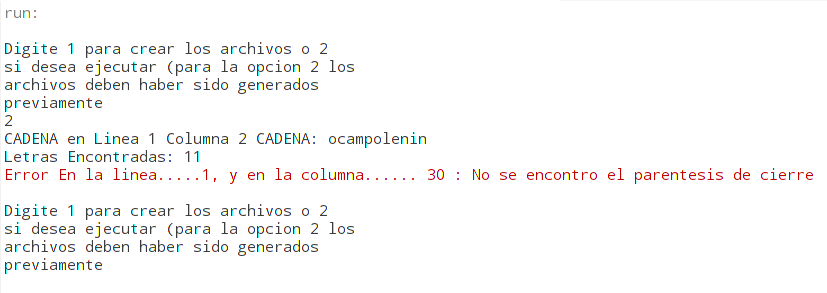
\includegraphics[height=0.25\textheight]{error.png}
\\
Figura 14: Error sintáctico sin parentesis
\end{center}

En la figura 14: Se muestra la salida por consola del error sintáctico.\\

Linea1: Muestra que encontró una cadena en la linea1 Columna2 y el contenido de ese objeto es: ocampolenin\\

Linea2:  Muestra el numero de letras encontradas en la cadena, obtenidas con el método contarLetras() de la clase AnalizadorSintactico.java, en este caso las letras encontradas son 11.\\

Line3: Muestra el error sintáctico en la Linea 1 y Columna 30 y muestra un mensaje especifico utilizando el identificador del símbolo faltante, en este caso dice que no se encontró el paréntesis de cierre.
\\

\textbf{Error sintáctico sin fin de linea}

\begin{center}
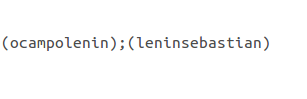
\includegraphics[height=0.11\textheight]{error2entrada.png}
\\
Figura 15: Entrada error sintáctico sin ; fin de linea
\end{center}

En la figura 15: Se muestra la entrada o la cadena ingresada la cual tiene un error sintáctico, falta el simbolo de fin de linea ; y como se especifico en las expresiones regulares cuyo formato es la cadena entre paréntesis y por ultimo un símbolo ; para especificar el final de la cadena. En este caso se observa que la segunda cadena no tiene  el punto y coma final, por lo tanto imprimirá un mensaje con el error sintáctico y adicional la linea y columna del error. 

\begin{center}
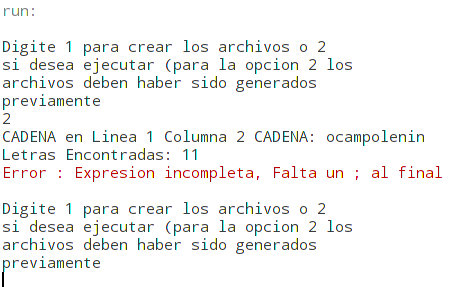
\includegraphics[height=0.3\textheight]{error2.png}
\\
Figura 16: Error sintáctico sin parentesis
\end{center}

En la figura 16: Se muestra la salida por consola del error sintáctico.\\

Linea1: Muestra que encontró una cadena en la linea1 Columna2 y el contenido de ese objeto es: ocampolenin\\

Linea2:  Muestra el numero de letras encontradas en la cadena, obtenidas con el método contarLetras() de la clase AnalizadorSintactico.java, en este caso las letras encontradas son 11.\\

Line3: Muestra el error sintáctico en la Linea 1 y Columna 31 y muestra un mensaje especifico utilizando el identificador del símbolo faltante, en este caso dice que no se encontró el fin de linea.


\newpage
\section{Links del Repositorio}

\subsection{Código Fuente: Compilador y Documento en Latex}

\textbf{GitHub: } \url{}.

\subsection{Repositorio de archivos academicos }

\textbf{Slideshare: } \url{}.

\newpage
\section{Conclusiones}

\begin{itemize}

\item La herramienta JFlex es una gran alternativa para comprender la relación que tienen los lenguajes formales y teoría de autómatas con las ciencias de la computación, ya que mediante la aplicación de estos conocimientos podemos crear nuestro propio lenguaje y expresiones regulares, que serán validadas utilizando el computador.
\item La utlización de expresiones regulares nos pueden ayudar a definir de forma exacta los lenguajes que utilizamos en la creación de los autómatas y con esto estructurar sin problemas el archivo .cup.

\item Las expresones regulares sirven como lenguajes de entrada de muchos sistemas que operan con cadenas, entre los mas comunes que utilizan estos tenemos los lenguajes de programación y los motores de busqueda.
\end{itemize}




\newpage
\section{Bibliografía}

\begin{thebibliography}{20}


\bibitem{1} 
Integración de Jflex y Cup (Analizadores léxico y sintáctico), Rafael A. Vega Castro, Octubre de 2008, Disponible en: \url{http://www.rafaelvega.info/wp-content/uploads/Articulo.pdf}.

\bibitem{2} 
Universidad Carlos III de Madrid, Breve Introducción a CUP, Disponible en: \url{http://www.it.uc3m.es/~luis/fo1/p/CUP.html}.


\end{thebibliography}

\end{document}
